\section{Generalizations}

The example presented is just an application to cyclic graph, also the components presented, the walker, 
the coin and the shift operator are meant to be generic. This method in fact can fit different type of problems and graph.
Starting from the coin there are many others operator that we can use, which are symmetrical, other examples are the 
balanced coins that get rid of asymmetrical behavior of the Hadamard coin. For more details
about different coins an introductory summary can be found in \cite{Kempe_2003}, but there are also Quantum walks without
the coin, as it is mentioned in \cite{6812670}.

% generalization for the graphs

The interesting thing is that the example presented can be adapted to a variety of other graphs, for instance we can
build a circuit able to perform a quantum walks also for complete graphs, hypercube, glued trees and others. 
Obviously, changing the graph, the circuit needs to be adapted but the idea remains the same. A very useful
references that shows circuits for the type of graphs mentioned is \cite{douglas2007efficient}

% multi controlled toffoli remark

An important remark concern the total qubits needed, as mentioned in the previous section if
the number of qubits is greater than 2 we need to use multi toffoli gate, this gates can be 
obtained by combining several toffoli gates, with the help of some ancillary qubits, those 
ancillary qubits are needed just to construct the multi controlled toffoli. In Fig. 5 below
is showed how to implement a multi controlled toffoli gates with 5 controls qubits, 
this image is taken from \cite{nielsen_chuang_2010}. In general following this procedure
we need a number of ancillary equals to controls qubits - 1.

\begin{figure}[h!]
    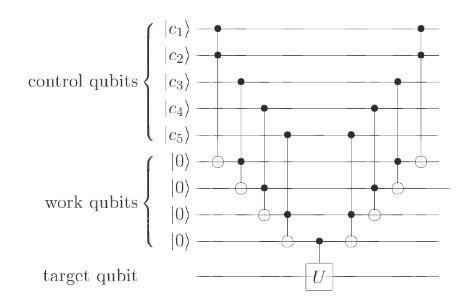
\includegraphics[scale=0.5]{img/ancillary.jpg}
    \caption{Practical representation of multi toffoli gate}
    \centering
\end{figure}

The number of ancillary qubits impacts also in the efficiency of the circuit. In the next
section will be provided a more formal description of efficiency.
